\section{Lecture 5:\\ Variational circuits}
\SectionPage{}

\begin{frame}{Variational Quantum Classifier}
    
A variational quantum circuit contains parameterized gates whose values depend on some variables $\theta_1, ..., \theta_n$.

\begin{enumerate}
    \item Instantiate the circuit choosing random $\theta$s;
    \item Run the circuit and obtain output $y$;
    \item Use $y$ to compute a loss function and update $\theta$s accordingly.
\end{enumerate}

\bigskip\alert{Advantage}: The iterative optimization of the parameters allows us to circumvent the high-depth circuit.

\medskip\structure{Disadvantage}: No assurance of speedup. 
\end{frame}





\begin{frame}{Variational Quantum Classifier (2)}

\begin{center}
    \begin{quantikz}
    \lstick[wires=3]{$\ket{0}$} 
    & \gate[wires=3][2cm]{U(x)} & \gate[wires=3][2cm]{U(\theta)} & \meter{} \rstick[wires=3]{$y$} \\
    & \qw & \qw & \meter{}  \\
    & \qw & \qw & \meter{}  \\
    \end{quantikz}
\end{center}

\begin{itemize}
    \item input $x \in \mathbb{R}^n$ is encoded through \emph{feature map} $U(x)$;
    \item the state evolves through variational form $U(\theta)$;
    \item the parameters $\theta$s are chosen to minimize a certain loss function.
\end{itemize}

\end{frame}




\begin{frame}{Variational Quantum Classifier (3)}

Any variational circuit is a QNN. 
\begin{itemize}
    \item Mathematically, a QNN is a rather different object compared to classical NN;
    \item the analogy refers to:
    \begin{itemize}
        \item ``modular" nature of quantum gates in a circuit;
        \item use of tricks from training neural networks in the optimization of quantum algorithms.
    \end{itemize}
\end{itemize}

\begin{center}
    \scalebox{0.9}{
    \begin{quantikz}
        \qw
            & \gate{RY(\theta_1)} \gategroup[wires=3,steps=4,style={inner sep=-0.2pt}]{hidden layer 1}
            & \ctrl{1}           
            & \ctrl{2} 
            & \qw
            & \gate{RY(\theta_4)} \gategroup[wires=3,steps=4,style={inner sep=-0.2pt}]{hidden layer 2}
            & \ctrl{1}           
            & \ctrl{2} 
            & \qw 
            & \qw \\
        \qw 
            & \gate{RY(\theta_2)} 
            & \targ{}  
            & \qw      
            & \ctrl{1}
            & \gate{RY(\theta_5)} 
            & \targ{}  
            & \qw      
            & \ctrl{1}
            & \qw \\
        \qw 
            & \gate{RY(\theta_3)} 
            & \qw      
            & \targ{}  
            & \targ{}
            & \gate{RY(\theta_6)} 
            & \qw      
            & \targ{}  
            & \targ{}
            & \qw 
    \end{quantikz}}
\end{center}

\end{frame}


\begin{frame}{Barren plateau}

\begin{block}{Barren Plateau}
When minimizing the cost function, we might have exponentially vanishing gradients, known as barren plateau landscapes. In that case, the network cannot be efficiently trained.
\end{block}

\begin{itemize}
    \item Depends on the network architecture (Cerezo et al., 2020);
    \item Depends on the feature map (Abbas et al., 2020). 
\end{itemize}
\end{frame}


\begin{frame}[fragile]{Your turn!}
Try the VQC. \bigskip

\begin{minted}{python}
IRIS_FEATURES = 4
optimizer = ADAM(maxiter=100, lr=0.1)
feature_map = ZZFeatureMap(feature_dimension=IRIS_FEATURES)
var_form = TwoLocal(IRIS_FEATURES)
vqc = VQC(optimizer, feature_map, var_form, 
    training_input, test_input)

backend = Aer.get_backend('statevector_simulator')
quantum_instance = QuantumInstance(backend, shots=1)
result = vqc.run(quantum_instance)
\end{minted}
\end{frame}


\section{Lecture 5:\\ Hadamard classifier}
\SectionPage{}

%\begin{frame}{The problem}
%Facial Expression Recognition (FER) is an extremely relevant task associated with human-computer interaction, with applications in predictive environments, content analysis, support for healthcare, and many more. 

%\bigskip FER is a classification problem, in which each picture representing a face have to be associated with its expression.

%\bigskip It is possible to solve FER with supervised learning approaches starting from a dataset for labelled pictures.
%\end{frame}



%\begin{frame}{The problem (2)}
%FER is solved using a quantum circuit that encodes:
%\begin{itemize}
%    \item a subset of the dataset;
%    \item the unlabelled test instance
%\end{itemize} 
%into quantum states.

%\bigskip Then, infer the test label as the one of the closest item in terms of Euclidian distance.
%\end{frame}


%\begin{frame}{The dataset}

The Extended Cohn-Kanade contains pictures from 123 different people from 18 to 50 years.

\bigskip 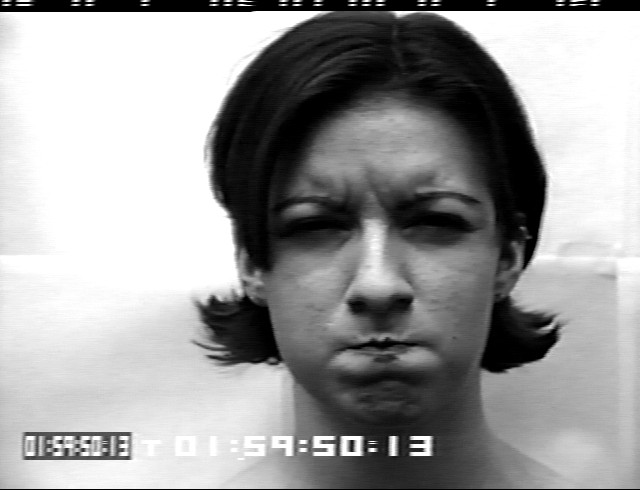
\includegraphics[width=.48\textwidth]{img/lec5f/S010_004_00000019.png}%
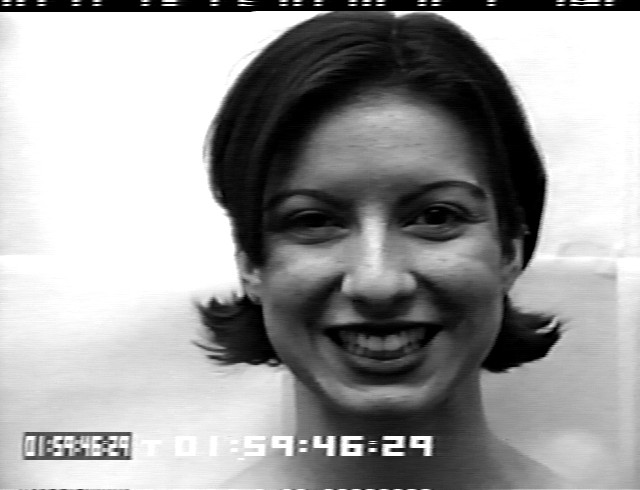
\includegraphics[width=.48\textwidth]{img/lec5f/S010_006_00000015.png}

\bigskip Each picture is labelled with one of the following emotion: anger, contempt, disgust, fear, happiness, sadness, and surprise.
    
\end{frame}
%\begin{frame}{Active Appearance Models}

Each pictures is processed with Active Appearance Models.

\bigskip Consider a cloud of 68 points representing some abstract face, in which each point (\emph{landmark point}) is some particular point of the face.

\bigskip\centering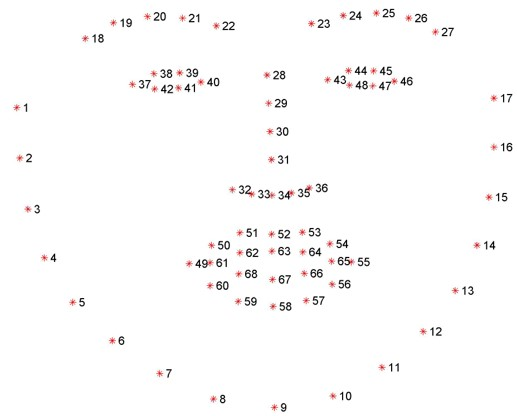
\includegraphics[width=.5\textwidth]{img/lec5f/template.jpg}
\end{frame}

\begin{frame}{Active Appearance Models (2)}
The cloud of points is deformed in order to stick with the face in the picture.

\bigskip\centering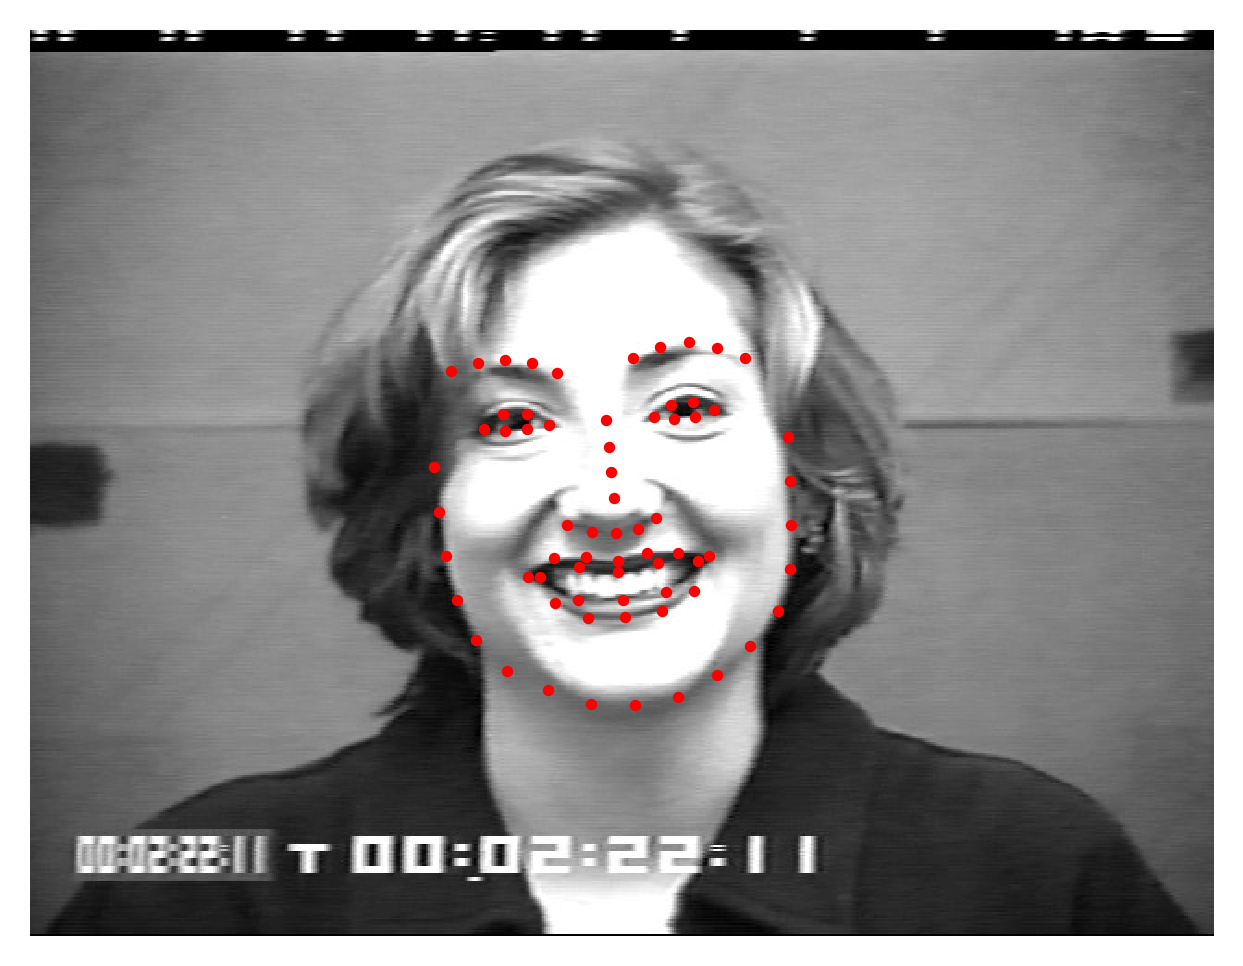
\includegraphics[width=.6\textwidth]{img/lec5f/S046_005_00000023.png}
\end{frame}
%\begin{frame}{Faces \(\to\) graphs}

We keep only point related to the mouth. 

\bigskip In order to obtain a \textit{weighted graph} from the previous data cloud we opted for two different strategies:

\only<1>{

\begin{itemize}
	\item \textbf{Complete graph} whose vertices are the landmark points of the mouth and  edge-weights $ w_{ij} $ are equal to  the Euclidean distance between vertices $ i $ and $ j $.
\end{itemize}	

\bigskip\centering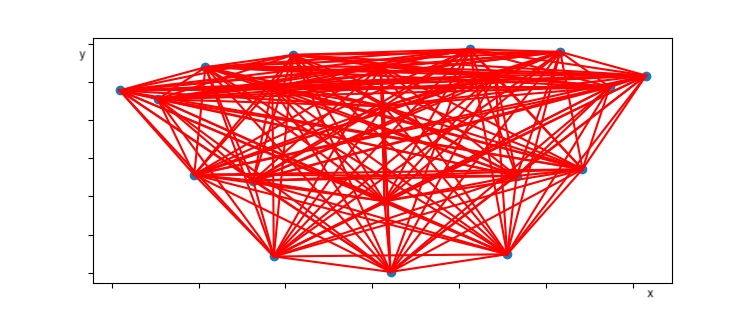
\includegraphics[width=0.5\textwidth]{img/lec5f/boccacomplete.png}}

\only<2>{

\begin{itemize}
	\item \textbf{Meshed graph} obtained using  the Delaunay triangulation algorithm of the  mouth  landmark points (complexity $ O(n \log n) $), also in this case the   edge-weights $ w_{ij} $ are equal to  the Euclidean distance between vertices $ i $ and $ j $.
\end{itemize}	

\bigskip\centering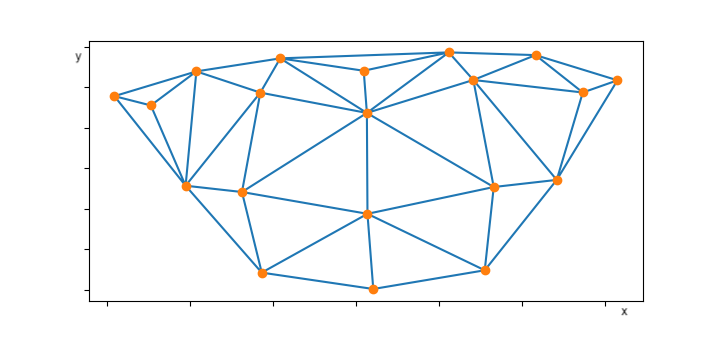
\includegraphics[width=0.5\textwidth]{img/lec5f/boccamesh.png}}

\end{frame}

\begin{frame}{Graph representation}

The graph is represented through its adjacency matrix.

\bigskip We keep only the upper triangular without diagonal, since the graph is undirected (symmetric matrix) and without self loop (the distance between any point with itself is zero). 

\bigskip Vectorize the matrix.

\end{frame}
\begin{frame}{Classical classifier}

The classifier receives in input the vector $x_\text{test}$ and two vectors $x_0, x_1$ which are one representative of the happy and sad faces.

\bigskip The Euclidian distances $\mathrm{distance}(x_\text{test}, x_0)$ and $\mathrm{distance}(x_\text{test}, x_1)$ are calculated. The test instance is classifies as the closest representative, whose distance is lower. 

\end{frame}

\begin{frame}[fragile]{The code}

\begin{minted}{python}
def classical_distance(G_0, G_1, G_test, tol=0.00001):
    
    # distance between the test instance and the happy instance
    distance_0 = np.linalg.norm(G_0 - G_test)
    # distance between the test instance and the sad instance
    distance_1 = np.linalg.norm(G_1 - G_test)
    # the difference is = 0 if the distance is equal, > 0 if sad is closest, < 0 if happy is closest
    difference = distance_0 - distance_1
    # remove some numerical error that can classify numbers like +-0.00001 as Y1 or Y0 instead of EQUALS
    the_difference = 0 if np.abs(difference) <= tol else difference
    
    # sign(difference) = 0 -> EQUAL; sign(difference) = 1 -> Y1; sign(difference) = -1 -> Y0
    label = int(np.sign(the_difference))
    return difference, ["EQUAL", "Y1", "Y0"][label]
\end{minted}
\end{frame}



\begin{frame}{Quantum classifier}
    \begin{center}
        \scalebox{0.8}{\begin{quantikz}[]
    \lstick{\(\ket{0}_a\)}\qw
        & \gate{H}
        & \ctrl{2}
        & \gate{X}
        & \ctrl{2}
        & \qw
        & \ctrl{2}
        & \gate{H}
        & \meter{\text{discard }1}
        & \cwbend{3}
        & \cw \rstick{a} \\
    \lstick{\(\ket{0}_i\)}\qw
        & \gate{H}
        & \qw
        & \qw
        & \ctrl{1}
        & \gate{X}
        & \ctrl{1} 
        & \ctrl{2}
        & \qw
        & \qw & \qw \\
    \lstick{\(\ket{0\cdots 00}_g\)}\qw
        & \qw
        & \gate{\mathbf{G_\text{\textbf test}}}
        & \qw
        & \gate{\mathbf{G^{\{1\}}}}
        & \qw
        & \gate{\mathbf{G^{\{2\}}}}
        & \qw
        & \qw
        & \qw & \qw \\
    \lstick{\(\ket{0}_c\)}\qw
        & \qw
        & \qw
        & \qw
        & \qw
        & \qw
        & \qw
        & \targ{}
        & \qw
        & \meter{}
        & \cw\rstick{c}
\end{quantikz}}
    \end{center}
\end{frame}

\begin{frame}{Quantum classifier}
The circuit evolves as it follows:
\only<1>{\begin{itemize}
\item the circuit starts in state:
$$|0\rangle_a |0\rangle_i |0\rangle_d |0\rangle_c;$$
\item after the first two Hadamard gates the state is:
$$\frac{1}{2} (|0\rangle+|1\rangle)_a (|0\rangle+|1\rangle)_i |0\rangle_d |0\rangle_c;$$
\end{itemize}
}%
%
\only<2>{\begin{itemize}
\item after the controlled initialization of the test instance the state is: 
$$\frac{1}{2} |0\rangle_a (|0\rangle+|1\rangle)_i |0\rangle_d |0\rangle_c
+ \frac{1}{2} |1\rangle_a (|0\rangle+|1\rangle)_i |G_\text{test}\rangle_d |0\rangle_c;$$
\item after the X operation on the ancilla qubit the state is:
$$\frac{1}{2} |0\rangle_a (|0\rangle+|1\rangle)_i |G_\text{test}\rangle_d |0\rangle_c
+ \frac{1}{2} |1\rangle_a (|0\rangle+|1\rangle)_i |0\rangle_d |0\rangle_c;$$
\end{itemize}
}%
%
\only<3>{\begin{itemize}
\item after the double-controlled initialization of the first representative the state is:
$$\frac{1}{2} |0\rangle_a (|0\rangle+|1\rangle)_i |G_\text{test}\rangle_d |0\rangle_c
+ \frac{1}{2} |1\rangle_a |0\rangle_i |0\rangle_d |0\rangle_c
+ \frac{1}{2} |1\rangle_a |1\rangle_i |G_0\rangle_d |0\rangle_c;$$
\item after the X operation on the index register the state is:
$$\frac{1}{2} |0\rangle_a (|0\rangle+|1\rangle)_i |G_\text{test}\rangle_d |0\rangle_c
+ \frac{1}{2} |1\rangle_a |0\rangle_i |G_0\rangle_d |0\rangle_c
+ \frac{1}{2} |1\rangle_a |1\rangle_i |0\rangle_d |0\rangle_c;$$
\item after the double-controlled initialization of the second representative the state is:
$$\frac{1}{2} |0\rangle_a (|0\rangle+|1\rangle)_i |G_\text{test}\rangle_d |0\rangle_c
+ \frac{1}{2} |1\rangle_a |0\rangle_i |G_0\rangle_d |0\rangle_c
+ \frac{1}{2} |1\rangle_a |1\rangle_i |G_1\rangle_d |0\rangle_c;$$
\end{itemize}
}%
%
\only<4>{\begin{itemize}
\item after the CNOT gate binding the index register with the class register, the state is:
{\footnotesize $$\frac{1}{2} |0\rangle_a |0\rangle_i |G_\text{test}\rangle_d |0\rangle_c
+ \frac{1}{2} |0\rangle_a |1\rangle_i |G_\text{test}\rangle_d |1\rangle_c
+ \frac{1}{2} |1\rangle_a |0\rangle_i |G_0\rangle_d |0\rangle_c
+ \frac{1}{2} |1\rangle_a |1\rangle_i |G_1\rangle_d |1\rangle_c;$$}%

for the sake of visualization, we set $|0\rangle_c$ as $|y_0\rangle_c$ and $|1\rangle_c$ as $|y_1\rangle_c$ to remind us that such register contains the two labels:
{\footnotesize $$\frac{1}{2} |0\rangle_a |0\rangle_i |G_\text{test}\rangle_d |y_0\rangle_c
+ \frac{1}{2} |0\rangle_a |1\rangle_i |G_\text{test}\rangle_d |y_1\rangle_c
+ \frac{1}{2} |1\rangle_a |0\rangle_i |G_0\rangle_d |y_0\rangle_c
+ \frac{1}{2} |1\rangle_a |1\rangle_i |G_1\rangle_d |y_1\rangle_c;$$}
which is re-arranged into the following equation:
$$ \frac{1}{2} \sum_{k \in \{0, 1\}} \Big( |0\rangle_a |G_\text{test}\rangle_d + |1\rangle_a |G_k\rangle_d  \Big) |k\rangle_i |y_k\rangle_c;$$
\end{itemize}
}%
%
\only<5>{\begin{itemize}
\item after the final Hadamard gate the state is: $$\frac{1}{2\sqrt{2}} \sum_{k \in \{0, 1\}} \Big( |0\rangle_a (|G_\text{test}\rangle + |G_k\rangle)_d + |1\rangle_a (|G_\text{test}\rangle - |G_k\rangle)_d \Big) |k\rangle_i |y_k\rangle_c.$$
\end{itemize}}
\end{frame}

\begin{frame}{Measurement interpretation}

By estimating the probability of reading class $y_0=0$ or $y_1=1$ we can estimate the distance between $G_\text{test}, G_0$ with respect to the distance between $G_\text{test}, G_1$. So, 

$$y_\text{test} = \begin{cases}
    y_0,           & > .5 \\
    y_1,           & < .5 \\
    \text{equals}, & = .5
\end{cases}$$

To mitigate the errors due to the probabilistic nature of the computation, we can introduce a small tollerance $\epsilon$ around the boundary between the two labels:

$$y_\text{test} = \begin{cases}
    y_0, & > .5+\epsilon \\
    y_1, & < .5-\epsilon \\
    \text{equals}, & \text{otherwise}
\end{cases}$$
\end{frame}
\begin{frame}[fragile]{Your turn!}
\begin{minted}{python}
def quantum_distance(G_0, G_1, G_test, tol=0.00001):
    # ...
    return difference, label
\end{minted}
\end{frame}

\begin{frame}[fragile]{Test the correctness}
\begin{minted}{python}
def test_accuracy_of_classification(states):
    correct, wrong = 0, 0
    for i, first_data in enumerate(states):
        for j, second_data in enumerate(states):
            for k, third_data in enumerate(states):
                dc, cl = classical_distance(first_data,
                    second_data, third_data)
                dq, ql = quantum_distance(first_data,
                    second_data, third_data, tol=0.015)
                if cl == ql:
                    correct += 1
                    print(".", end="")
                else:
                    wrong += 1
                    print("X", end="")
    return (correct, wrong)
\end{minted}
\end{frame}

\begin{frame}[fragile]{Test the correctness}
\begin{minted}{python}
# create some quantum states
zero  = np.array([1, 0])
one   = np.array([0, 1])
plus  = (1/np.sqrt(2)) * np.array([1, 1])
minus = (1/np.sqrt(2)) * np.array([1, -1])
ipos  = (1/np.sqrt(2)) * np.array([1, complex(0,1)])
ineg  = (1/np.sqrt(2)) * np.array([1, complex(0,-1)])

# run the test
states = [zero, one, plus, minus, ipos, ineg]
correct, wrong = test_accuracy_of_classification(states)

# print results
print(f"\nClassified {correct} correctly and {wrong} wrongly")
\end{minted}
\end{frame}

\begin{frame}{Your turn!}
Download the starter code. The file \code{dataset.json} contains 26 elements, representing the path of an image, a path of its file containing the landmark points and its label. 

\bigskip Estimate the accuracy of both classical and quantum classifier. 
\end{frame}